\chapter{Application mobile}

	\section{API REST}

		\subsection{Organisation des packages}

			%TODO Léa : Image et décrire le but des packages (src)
			L'organisation des packages se déroule comme suit :

			\begin{figure}[H]
				\centering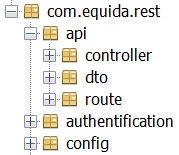
\includegraphics[width=0.33\textwidth, keepaspectratio]{res/package.png}
				\caption{Packages de l'api Rest}
			\end{figure}

			\begin{description}
				\item[api :]{Contient les fichiers de l'api}
				\begin{description}
					\item[controller :]{Contient tous les controleurs}
					\item[dto :]{Contient tous les Dto}
					\item[route :]{Contient toutes les routes}
				\end{description}
				\item[authentification :]{Contient la classe qui implémente BasicAuthenticationEntryPoint pour configurer Basic Authentification sur l'application}
				\item[config :]{Contient les classes de configuration et de sécurisation de l'application}
			\end{description}

		\subsection{Parler configuration de l'application}

			\subsubsection{application.properties}

				%TODO Justine

			\subsubsection{Configuration par le code}

				%TODO Justine

		\subsection{Parler authentification}

			%TODO Justine

		\subsection{Exemple Route}

			%TODO Léa : Expliquer les méthodes de l'interface IRoute et donner un exemple de route.
			L'interface IRoute décrit la méthode qui doit être implémentée par les classes filles.\newline
			Ainsi chaque fichier route contiendra une méthode getUri() qui retournera l'URL à utiliser dans la page concernée (pour la route correspondante).

			\noindent
			Par exemple, pour LotsApiRoute, qui est donc la route principale de l'api pour la gestion des lots selon notre nomenclature, l'URL renvoyée est /api/lots.

			\begin{figure}[H]
				\centering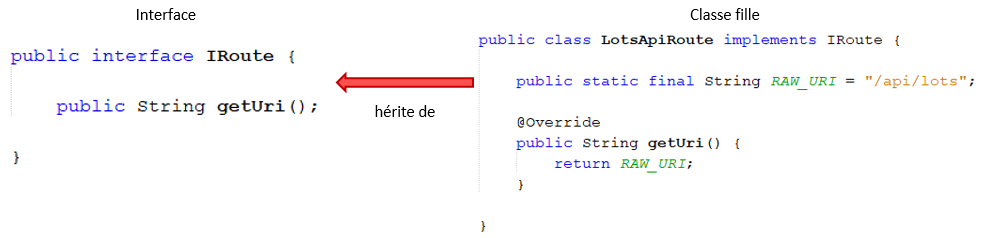
\includegraphics[width=0.80\textwidth, keepaspectratio]{res/IRoute.png}
				\caption{Interface IRoute et exemple avec LotsApiRoute}
			\end{figure}


		\subsection{Exemple Dto}

			%TODO Justine : Expliquer interface IDto
			%TODO JU : TU PEUX GERER L'EXEMPLE GENRE AVEC CHEVAL ET EXPLIQUER CONVERTTODTO ET CONVERTOENTITY ?


		\subsection{Exemple Controller}

			%TODO Léa : Donner un exemple de controller
			Les différents contrôleurs sont des classes précédées de l'annotation @RestController. \newline
			Les contrôleurs contiennent différentes méthodes associées aux méthodes GET, POST, PATCH et DELETE ainsi qu'a une route. Enfin elles utilisent les services pour intéragir avec la \bdd{}. On y définit aussi les différentes autorisations avec l'annotation @PreAuthorize afin de savoir qui peut accéder à la page, et donc, executer la méthode.

			\noindent
			Par exemple, pour LotDetailsRestController, on implémente la méthode getLot, liée à la route LotDetailsApiRoute.RAW\_URI, qui prend en paramètre l'id du lot concerné. Elle va retourner (grâce à la méthode getById de LotService) le lot correspondant sous la forme d'un LotDto.

			\begin{figure}[H]
				\centering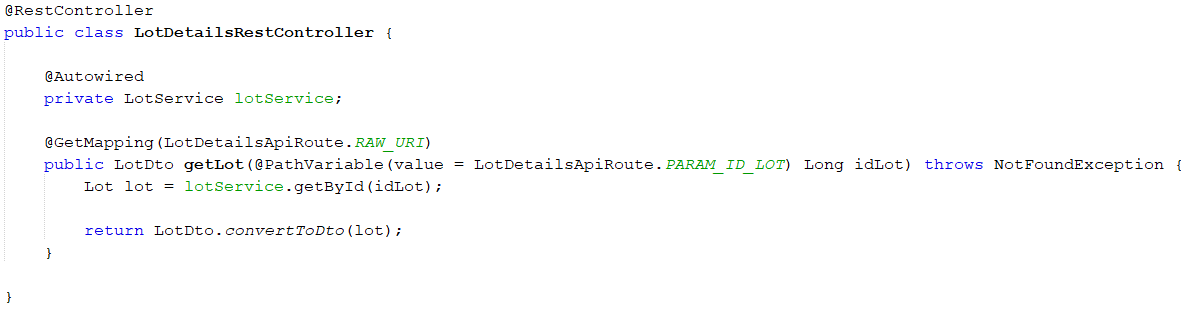
\includegraphics[width=0.80\textwidth, keepaspectratio]{res/lotsController.png}
				\caption{Exemple d'un contrôleur avec LotDetailsRestController}
			\end{figure}


	\section{Ionic}

		\subsection{Organisation des packages}

			%TODO Léa : Image et décrire le but des packages (src)
			L'organisation des packages se déroule comme suit :

			\begin{figure}[H]
				\centering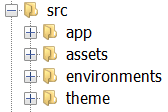
\includegraphics[width=0.33\textwidth, keepaspectratio]{res/ionicPackage.png}
				\caption{Packages de ionic}
			\end{figure}

			\begin{description}
				\item[app :]{Contient les fichiers de l'applicaton}
				\item[assets :]{Contient les images de l'applications}
				\item[environments :]{Contient les différents "mode de fonctionnement" de l'application. On aura par exemple un environment de développement (utilisé par défaut) ainsi qu'un autre pour faire fonctionner l'application en mode production. On pourra ainsi affiner le nieau de debug et de log pour voir, ou non plus d'erreur et intégrer des outils pour simplifier le débugguage d e l'application.}
				\item[theme :]{Contient le fichier variables.scss qui définit les couleurs utilisées par ionic}
			\end{description}

		\subsection{Les pages}

			%TODO Léa : Parler de la nommenclature
			Les différentes pages générées (via la commande "ionic g") suivent la même nomenclature : elles sont placées dans un dossier du nom de l'entité concernée suivit d'un verbe (souvent : lister, ajouter, consulter, modifier). \newline

			\begin{figure}[H]
				\centering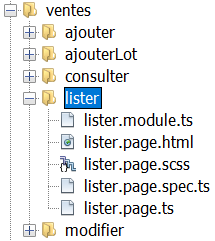
\includegraphics[width=0.33\textwidth, keepaspectratio]{res/ionicListerVentes.png}
				\caption{Résultat de la commande "ionic g" avec un nom de page correspondant à lister dans le dossier ventes}
			\end{figure}

			Dans chaque sous-dossier (un sous-dossier pour lister, un pour ajouter, ...) créé par la commande ionic, on retrouvera les mêmes types de fichiers.\newline

			\begin{description}
				\item[x.module.ts :]{Exporte notre module pour être utilisable par Ionic}
				\item[x.page.html :]{Contient le code HTML de la page ainsi que les composants ionic}
				\item[x.page.scss :]{Permet de modifier le style de la page}
				\item[x.page.spec.ts :]{Permet d'effectuer des tests unitaires}
				\item[x.page.ts :]{Contient toutes les méthodes à éxécuter ainsi que l'initialisation de la page}
			\end{description}

			On ne travaillera que sur les fichiers x.page.ts, x.page.html.

			\subsubsection{Lister}

					%TODO Léa : Donner un exemple
					La page lister.page.html, contient donc un header avec le titre de la page ; ainsi qu'un content avec la liste et une boucle permettant l'affichage des ventes (*ngFor="let v of ventes") et la gestion d'un clic sur une vente (routerLink="/ventes/{{v.id}}") qui renvoie donc sur la page de la vente en question. \newline
					On retrouve aussi un test sur le role de l'utilisateur (*ngIf="role == 'ADMIN'"), si l'utilisateur a un role 'ADMIN' alors il verra un bouton flottant d'ajout. Ce bouton le renverra vers la page d'ajout d'une vente. \newline
					Pour finir, on affiche plus de ventes sur la page lors d'un scroll de l'utilisateur si celui ci atteind le bas de la page.

					\begin{figure}[H]
						\centering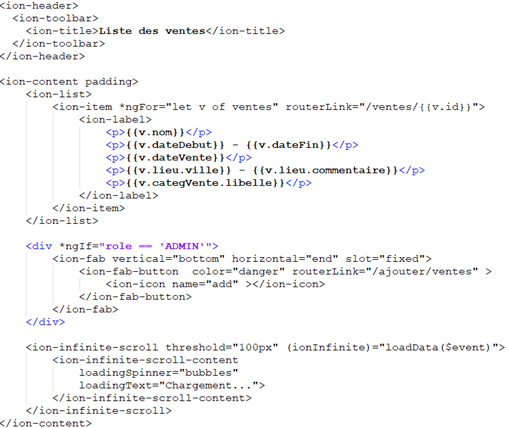
\includegraphics[width=0.9\textwidth, keepaspectratio]{res/lister.png}
						\caption{Code de /ventes/lister/lister.page.html}
					\end{figure}

					La page lister.page.ts, contient le constructeur, l'initialisation des variables, l'initialisation de la page avec la méthode ngOnInit qui appelle notamment la méthode getVentes. Cette méthode appelle la méthode loadVentes qui chargera donc les ventes, pour peux qu'il en reste à récupérer (et qui récupèrera le lieu et la catégorie de vente, par leur id respectif, afin de les afficher).

					\begin{figure}[H]
						\centering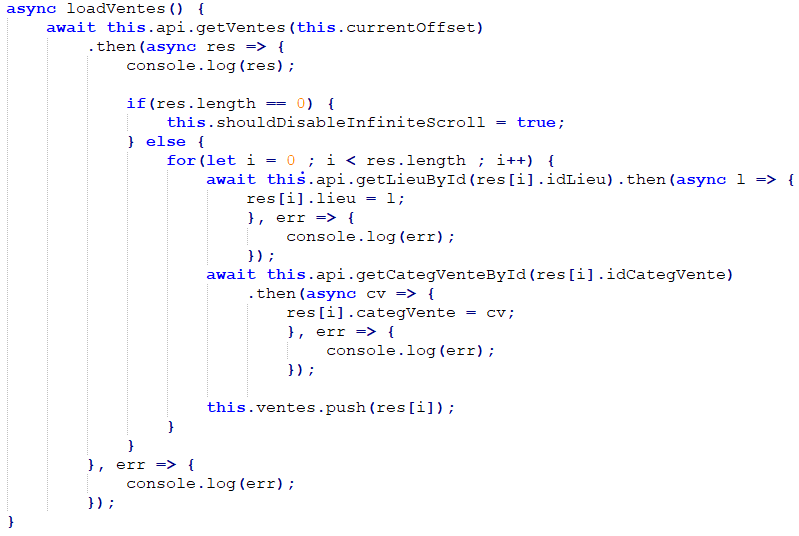
\includegraphics[width=0.9\textwidth, keepaspectratio]{res/listerTs.png}
						\caption{Code méthode loadVentes de /ventes/lister/lister.page.ts}
					\end{figure}

					\begin{figure}[H]
						\centering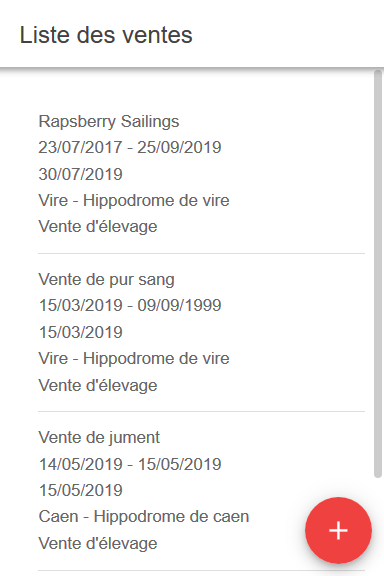
\includegraphics[width=0.33\textwidth, keepaspectratio]{res/listerVentes.png}
						\caption{Résultat de la page lister les ventes}
					\end{figure}

			\subsubsection{Consulter}

			%TODO Léa : Donner un exemple
			La page consulter.page.html, contient donc un header avec le titre de la page ; ainsi qu'un content avec un composant ionic card (purement visuel) dans lequel on retrouve des items correspondant aux différents champs d'une vente.\newline
			Puisque c'est une page de consultation, les champs affichent les valeurs contenues dans la base de données.\newline
			On trouve, là-aussi des boutons. Un pour proposer un cheval, seulement disponible pour un utilisateur classique ainsi que des boutons pour modifier et supprimer, tous deux présents seulement si l'utilisateur connecté est un administrateur. \newline
			Sur le même principe, on a aussi la liste des lots en vente (que l'on affiche pas ci-dessous dans le code mais qui est présent dans le fichier).

			\begin{figure}[H]
				\centering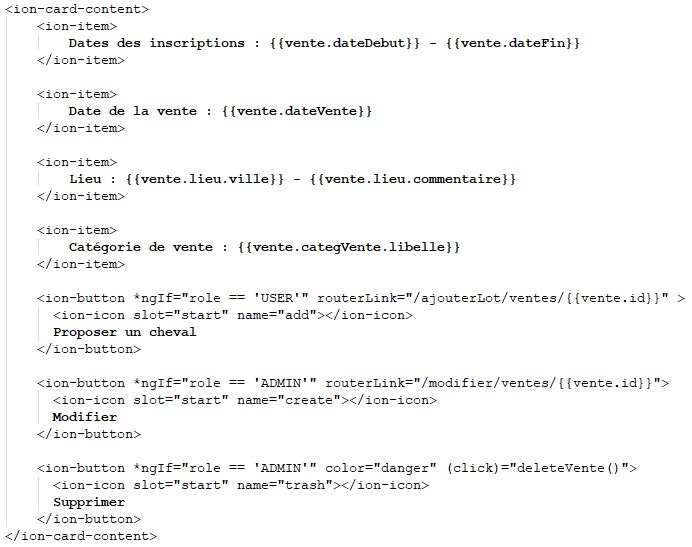
\includegraphics[width=0.9\textwidth, keepaspectratio]{res/consulter.png}
				\caption{Extrait du code de /ventes/consulter/consulter.page.html}
			\end{figure}

			La page consulter.page.ts, contient le constructeur, l'initialisation des variables, l'initialisation de la page avec la méthode ngOnInit qui appelle notamment les méthodes getVenteById et getLotsByIdVente.\newline
			La méthode getVenteById se charge donc de récupérer la vente par l'id passé en paramètre de la route. Afin d'afficher le lieu et la catégorie de vente, elle utilise aussi les méthodes getLieuById et getCategVenteById de l'api qui renvoient le bon nom, libellé en fonction de l'id fourni par la vente affichée.\newline
			On trouve aussi la méthode deleteVente appelée lors du clic sur le bouton supprimer. La vente dont l'id est passé en paramètre sera supprimée et l'utilisateur sera redirigé vers les pages des ventes.

			\begin{figure}[H]
				\centering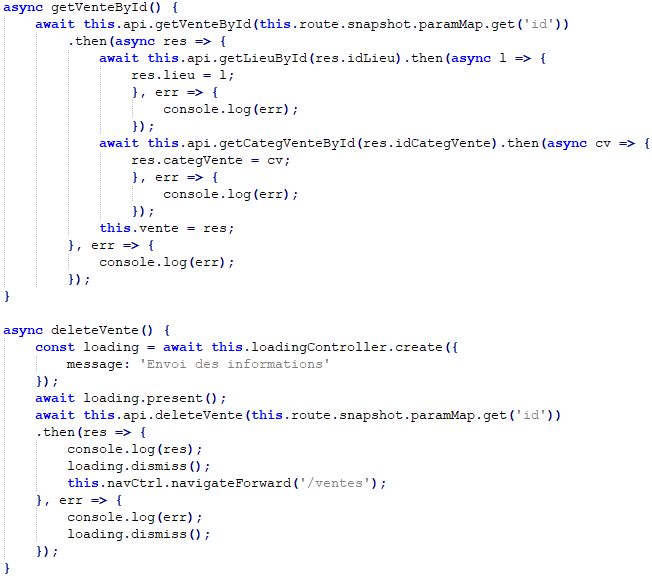
\includegraphics[width=0.9\textwidth, keepaspectratio]{res/consulterTs.png}
				\caption{Extrait du code de /ventes/consulter/consulter.page.ts}
			\end{figure}

			\begin{figure}[H]
				\centering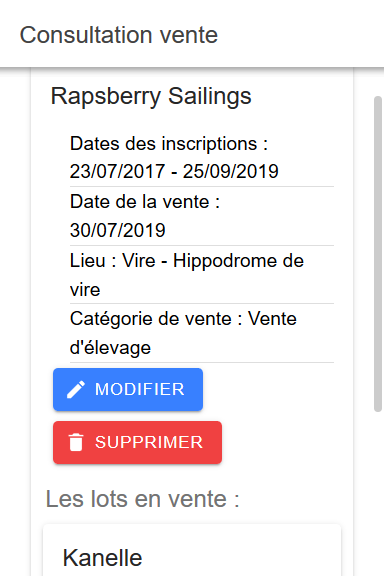
\includegraphics[width=0.33\textwidth, keepaspectratio]{res/consulterVente.png}
				\caption{Résultat de la page de consultation d'une vente}
			\end{figure}

			\subsubsection{Ajouter}
			%TODO Léa : Donner un exemple
			La page ajouter.page.html, contient donc un header avec le titre de la page ; ainsi qu'un content avec les différents items et input. \newline
			Dans les input et les select, on retrouve [(ngModel="nomChamp")] qui fera donc le lien entre les données saisies dans ce champ et les variables associées.\newline
			On a aussi un bouton qui lorsqu'il est cliqué, appelle la méthode addVente.

			\begin{figure}[H]
				\centering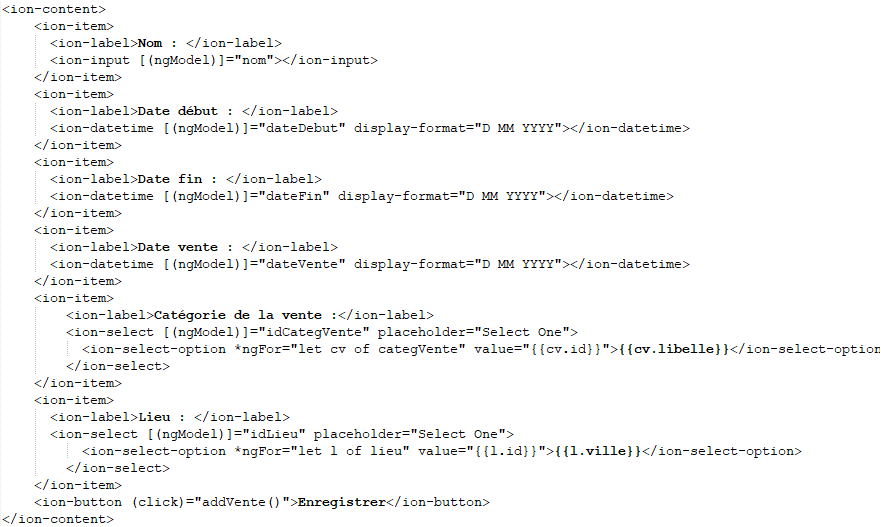
\includegraphics[width=0.9\textwidth, keepaspectratio]{res/ajouter.png}
				\caption{Code de /ventes/ajouter/ajouter.page.html}
			\end{figure}

			La page ajouter.page.ts, contient le constructeur, l'initialisation des variables, l'initialisation de la page avec la méthode ngOnInit qui appelle notamment les méthodes getCategVente et getLieux de l'api.\newline
			La méthode addVente se chargera donc de créer la vente grâce aux paramètres passés dans la méthode de l'api.

			\begin{figure}[H]
				\centering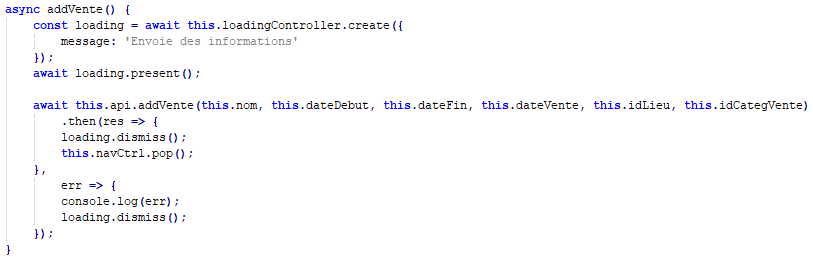
\includegraphics[width=0.9\textwidth, keepaspectratio]{res/ajouterTs.png}
				\caption{Extrait du code de /ventes/ajouter/ajouter.page.ts}
			\end{figure}

			\begin{figure}[H]
				\centering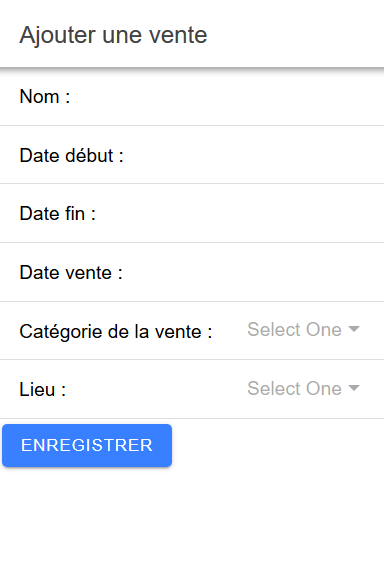
\includegraphics[width=0.33\textwidth, keepaspectratio]{res/ajouterVente.png}
				\caption{Résultat de la page d'ajout d'une vente}
			\end{figure}

			\subsubsection{Modifier}

			%TODO Léa : Donner un exemple
			La page modifier.page.html, est sensiblement la même que ajouter.page.ts. A la différence que le bouton, lorsqu'il est cliqué, appelle la méthode updateVente.

			La page modifier.page.ts, contient le constructeur, l'initialisation des variables, l'initialisation de la page avec la méthode ngOnInit qui récupère les valeurs de la vente à modifier.\newline
			La méthode updateVente se chargera donc de modifier la vente grâce aux paramètres passés dans la méthode de l'api.

			\begin{figure}[H]
				\centering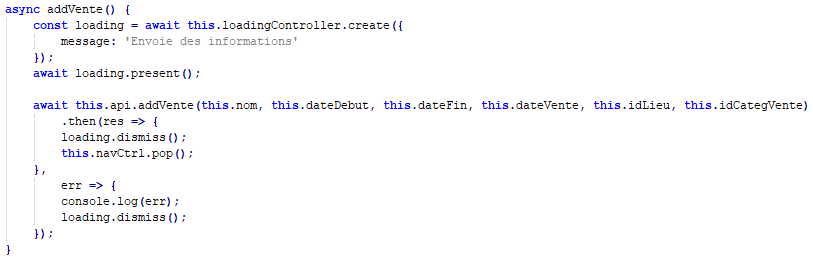
\includegraphics[width=0.9\textwidth, keepaspectratio]{res/ajouterTs.png}
				\caption{Extrait du code de /ventes/modifier/modifier.page.ts}
			\end{figure}

			\begin{figure}[H]
				\centering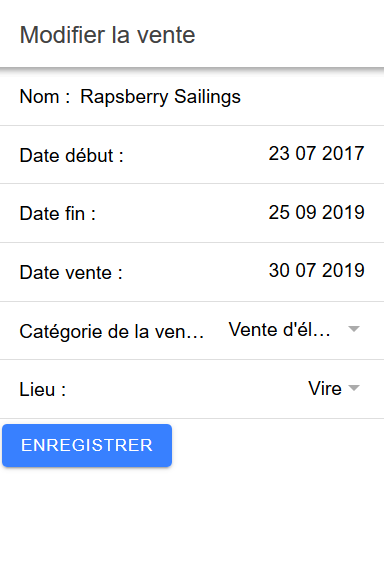
\includegraphics[width=0.33\textwidth, keepaspectratio]{res/modifierVente.png}
				\caption{Résultat de la page de modification d'une vente}
			\end{figure}

		\subsection{Rest Api}

			%TODO Justine

		\subsection{Authentification à l'Api}

			%TODO Justine

		\subsection{Problèmes connus}

			%TODO Léa : Parler refresh si ajout ou modif
			Cette application mobile comporte des erreurs sur lesquelles nous n'avons pas pu, su intervenir. En effet, après un ajout ou une modification (quelque soit l'entité concernée), lorsque l'utilisateur est redirigé vers la page principale (celle qui liste), les informations ne sont pas mises à jour car la page n'est pas actualisée. \newline
			Afin de palier à cette erreur, il est nécessaire d'actualiser "manuellement" la page.

			%TODO Justine : Parler affichage message erreur sur le formulaire
